\documentclass[12pt,letterpaper]{article}
\title{An Exploration in Reachability}
\usepackage[utf8]{inputenc}
\usepackage[framed,numbered]{matlab-prettifier}
\let\ph\snippetPlaceholder
\lstset
{
  style = Matlab-editor,
  escapechar      = ",
}
\usepackage{graphicx}
\usepackage{subfig}


\usepackage{amsmath}
\usepackage{amssymb}
\usepackage{commath}
\usepackage{mathtools}


%Title Format
\usepackage{titlesec}
\usepackage{enumitem}
\titleformat*{\section}{\bfseries\large}
\titleformat*{\subsection}{\bfseries\normalsize}




%Modificación del formato de los captions
\usepackage[margin=10pt,labelfont=bf]{caption}

%Paquete para incluir comentarios
\usepackage{todonotes}

%Paquete para incluir hipervínculos
\usepackage[colorlinks=true, 
            linkcolor = blue,
            urlcolor  = blue,
            citecolor = black,
            anchorcolor = blue]{hyperref}

%%%%%%%%%%%%%%%%%%%%%%
%The Document%
%%%%%%%%%%%%%%%%%%%%%%

\begin{document}
\renewcommand{\labelitemi}{$\checkmark$}


\begin{center}
	\textbf{\LARGE{An Exploration in Reachability}}\\
	\vspace{7mm}
		\textbf{\large{DJ Passey}}\\

	\vspace{4mm}
	\textbf{\large{BYU Information and Decision Algorithms Laboratories}}\\
	\textbf{\large{Professor: Sean Warnick}}\\
	November 16th, 2017
\end{center}

\vspace{7mm}

\section{Introduction}

The concept of reachability is a key idea in control theory. In the following sections, we explore it's definition and implications, showing that while a system is reachable it may not be possible provide a minimum input that drives the system to follow a continuous curve. This is demonstrated through the analysis of two similar systems that exhibit very different behavior.

\section{What is reachability?}
\subsection{Definition}
A system is \textbf{reachable} if there exists a control signal, which transposes the system from an initial state to any designed final state.
\subsection{Characterizations}
There are several methods to determine if a system is reachable. Let $A$ be an $n$x$n$ matrix and let $B$ be an $n$x$q$ matrix. Then for the system $Ax + Bu$, the following are equivalent:

\begin{enumerate}
\item The system is reachable
\item The reachability matrix $R$, where
\[R = [\ A^{n-1}B\ |\ A^{n-2}B\ |\ \cdots \ |\ AB\ |\ B\ ] \]
is invertible.
\item The reachability grammian $W_{r}$ is invertible where
\[W_{r}=\int _{0}^{\infty} e^{A(\tau)}BB^{T}e^{A^{T}(\tau)}d\tau \]
for continuous time systems and
\[W_{r} = \sum_{k=1}^{\infty} (A)^{k}BB^{T}(A^{T})^{k}\]
for discrete time systems.
\item The matrix $[\ A-\lambda I\ |\ B\ ]$ has rank $n$ for some eigenvalue $\lambda$ of $A$.
\end{enumerate}
 Building on these characterizations, we will proceed with two examples of reachable systems.

\section{Example: Semi-stable System}
Let $A_{0} = \begin{bmatrix} 0 & 1 \\ 0 & 0 \end{bmatrix}$ and $B = \begin{bmatrix} 0 \\ 1 \end{bmatrix}$. \vspace{5mm} \\

\noindent We compute the reachability matrix \[R = [\  AB\ |\ B\ ] = \begin{bmatrix} 1 & 0 \\ 0 & 1 \end{bmatrix}\] and observe that it is invertible. This implies that the system $A_{0}x + Bu$ is reachable.\\

\noindent Next we will examine the following question: Can we solve for an input $u(t)$ that drives our systems states to follow the unit circle?

\subsection{Tracing the unit circle}
Having checked that the system is reachable, we know that we can drive the system states from any starting point to any ending point. For this example, we will attempt to drive our system states to follow the unit circle along the parameterization \[ x(t) = \begin{bmatrix} x_{1}(t) \\ x_{2}(t) \end{bmatrix} = \begin{bmatrix} cos(\omega t) \\ -sin(\omega t) \end{bmatrix} \] for some $\omega \in \mathbb{R}$. (We include $\omega$ in our parameterization to allow the solution input to trace the unit circle in an arbitrary amount of time.) \vspace{1em}

\noindent Assume an input $u(t)$ will drive the system to follow this parameterization. If it exists, we can solve for it as follows:
\[\dot{x}(t) = A_{0}x(t) + Bu(t)\]
\[\begin{bmatrix} -\omega sin(\omega t) \\ -\omega cos(\omega t) \end{bmatrix} = \begin{bmatrix} 0 & 1 \\ 0 & 0 \end{bmatrix} \begin{bmatrix} cos(\omega t) \\ -sin(\omega t) \end{bmatrix} + \begin{bmatrix} 0 \\ 1 \end{bmatrix} u(t) \]
\[\begin{bmatrix} -\omega sin(\omega t) \\ -\omega cos(\omega t) \end{bmatrix} =  \begin{bmatrix} -sin(\omega t) \\ u(t) \end{bmatrix} \]
Then, $\omega = 1$ and $u(t) = -cos(t)$. Thus, the input $u(t) = -cos(t)$ will drive the system states to trace the unit circle once for $t \in [0,2\pi]$.

\section{Example: Stable System}
While the semi-stable system can trace the unit circle, the following reachable system cannot.
\[ A_{1} = \begin{bmatrix} -1 & 1 \\ 0 & -1 \end{bmatrix}\  B = \begin{bmatrix} 0 \\ 1 \end{bmatrix}\]  \\

\noindent We compute the reachability matrix: \[R = [\  AB\ |\ B\ ] = \begin{bmatrix} 1 & -1 \\ 0 & 1 \end{bmatrix}\] This is also invertible. Then the system $A_{1}x + Bu$ is reachable as well. 

\subsection{Tracing the unit circle}
Assuming that there is some input $u(t)$ that drives the states of this system to follow the unit circle, we proceed as before.\\
\[\dot{x}(t) = A_{1}x(t) + Bu(t)\]
\[\begin{bmatrix} -\omega sin(\omega t) \\ -\omega cos(\omega t) \end{bmatrix} = \begin{bmatrix} -1 & 1 \\ 0 & -1 \end{bmatrix} \begin{bmatrix} cos(\omega t) \\ -sin(\omega t) \end{bmatrix} + \begin{bmatrix} 0 \\ 1 \end{bmatrix} u(t) \]
\[\begin{bmatrix} -\omega sin(\omega t) \\ -\omega cos(\omega t) \end{bmatrix} =  \begin{bmatrix} -cos(\omega t) -sin(\omega t) \\ sin(\omega t) + u(t) \end{bmatrix} \]
Equating the first components gives,
\[-\omega sin(\omega t) = -cos(\omega t) -sin(\omega t) \]
Equating the coefficients of $sin( \omega t)$ and $cos( \omega t)$ gives,
\[-\omega = -1\]
\[0 = -1\]
and we have arrived at a contradiction. This implies that there is no input $u(t)$ that drives the states of $A_{1}x+Bu$ to follow this parameterization of the unit circle. This seems to contradict reachability! It is true that we can drive the states of our system to whatever values we want, but somehow, in the case of $A_{1}$, we cannot follow the unit circle.

\section{Minimum Energy Input Sampling}
To investigate further we will take a new approach. Instead of solving directly for $u(t)$, we will construct it by concatenating many small inputs that drive the system from one point on the unit circle to another close neighbor.  Consider the set of $N$ evenly spaced, consecutive points, $\{p_{i}\}_{i=1}^{n}$ on the unit circle. By reachability of either of our systems, we can construct an input that will drive the system states from any $p_{k}$ to $p_{k+1}$ for $k=1,2,3,\cdots, n-1$. If we give our system an initial value $x(0) = p_{1}$, it is possible that our concatenation of inputs will drive the system to follow the circle. 

\subsection{Review of Minimum Energy Input Calculation}
To create our various input functions, we will solve for the minimum energy input. Recall that the relationship of $x(L)$ to $u(t)$ with initial value $x_{0}$ is,
\[ x(L) = e^{AL}x_{0} + \int_{0}^{L}e^{A(L-\tau)}Bu(\tau)\ d\tau \]
and the time $L$ reachability grammian is:
\[W_{r}(L)=\int _{0}^{L} e^{A(L-\tau)}BB^{T}e^{A^{T}(L-\tau)}d\tau \]
Let $x_{1}$ be the vector of desired state values. Since we are dealing with reachable systems, we know that the grammian is invertible. 
By setting 
\[u(t) = B^{T}e^{A^{T}(L-t)}W^{-1}(x_{1} - e^{A(L-t)}x_{0})\]
and plugging it in to the equation for $x(L)$ we find that
\[ x(L) = e^{A(L)}x_{0} + \int_{0}^{L}e^{A(L-\tau)}BB^{T}e^{A^{T}(L-\tau)}W_{r}^{-1}(L)(x_{1} - e^{A(L)}x_{0}) \ d\tau \]
\[ x(L) = e^{A(L)}x_{0} + W_{r}(L)W_{r}^{-1}(L)(x_{1} - e^{A(L)}x_{0}) \]
\[ x(L) = e^{A(L)}x_{0} + x_{1} - e^{A(L)}x_{0} \]
\[ x(L) = x_{1}\]
Thus, $u(t)$ as defined above drives the system from an initial state $x_{0}$ to any desired $x_{1}$ in time $L$. It can be shown that the $L_{\infty}$ norm of this input is equal to the minimum amount of energy it takes to drive the system states from $x_{0}$ to $x_{1}$.

\subsection{Driving the System in Matlab}
Using the input solution above, we can drive our system to trace the points $\{p_{i}\}_{i=1}^{n}$ consecutively. The following code creates the appropriate inputs and drives the system to trace $N$ points on the unit circle.

\begin{lstlisting}[caption={Driving a System to Follow the Unit Circle In Matlab}]
% Create the system object 
A0 = [ 0 1 ; 0 0];
B = [0 ; 1];
C = eye(2,2);
D = [0 ; 0];
SYS = ss(A0,B,C,D); 

N = 100; % Number of points to interpolate
T = 2*pi/N; % Length of time between points
Nvec = 0:N-1;
Xn = exp(-1i*Nvec*T); % N roots of unity
Xn = [real(Xn)' imag(Xn)' ]';
x0 = Xn(1,:)'; % Starting point
Xn = [Xn' x0] %I nclude x0 again at the end
res = 100; % Number of samples
U = []; % Empty Vector of inputs
t = linspace(0,T,res); % Time vector
Wr = [1/3*(T^3) .5*(T^2); .5*(T^2) T]; % Gramian
eAT = [ 1 T ; 0 1]; % Exponentiated Matrix

% Generate the inputs for the Semi-Stable System
Y = [];
for i = 2:N
    x1 = Xn(i,:)';
    Alpha = Wr\(x1 - eAT*x0); % Calculate Wr^-1(x1 - eATx0)
    u1 = zeros(1,res);
    for j = 1:res
        u1(j) = [T - t(j), 1 ]*Alpha; % Sample u(t)
    end
    states = lsim(SYS,u1,t,x0); % Drive the system
    Y = [Y ; states]; % Concatenate the states
    x0 = x1;
end
plot(Y(:,1),Y(:,2)) % Plot States
\end{lstlisting}
\pagebreak
\begin{figure}
\begin{tabular}{cc}
\subfloat[N = 2]{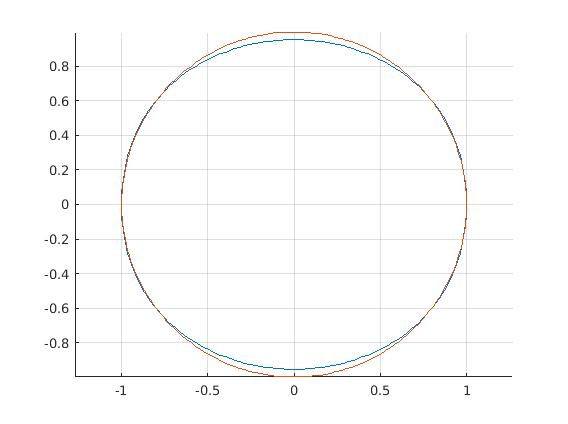
\includegraphics[width = 2.7in]{./unst2.jpg}} &
\subfloat[N = 3]{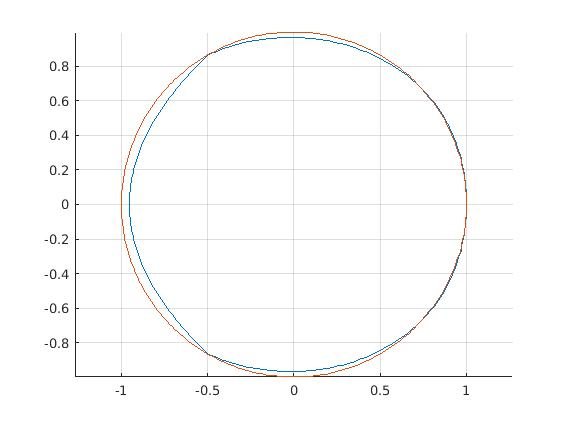
\includegraphics[width = 2.7in]{./unst3.jpg}} \\
\subfloat[N = 5]{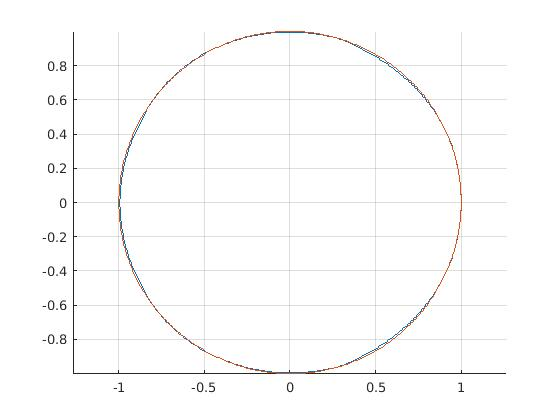
\includegraphics[width = 2.7in]{./unst5.jpg}} &
\subfloat[N = 10]{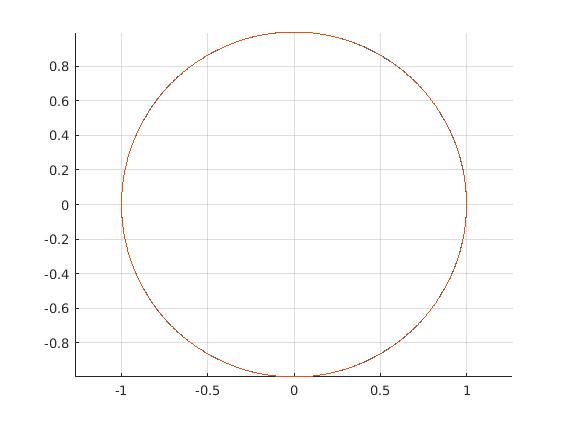
\includegraphics[width = 2.7in]{./unst10.jpg}}\\
\end{tabular}
\caption{}
\end{figure}
\subsection{Results of Simulation for the Semi-Stable System}
The above graphs show the system $A_{0}x + Bu$ as it is driven to interpolate $N$ points on the unit circle.  The unit circle is graphed in red and the system states are graphed in blue. Notice how as $N$ increases, the system states more closely adhere to the unit circle. Though not show here, we also found that as $N$ increases, the minimum energy input more closely approximates $-cos(t)$.

\pagebreak

\begin{figure}
\begin{tabular}{cc}
\subfloat[N = 2]{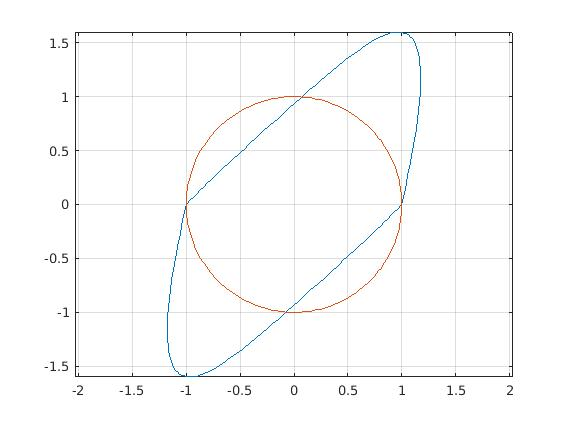
\includegraphics[width = 2.7in]{./stab2.jpg}} &
\subfloat[N = 5]{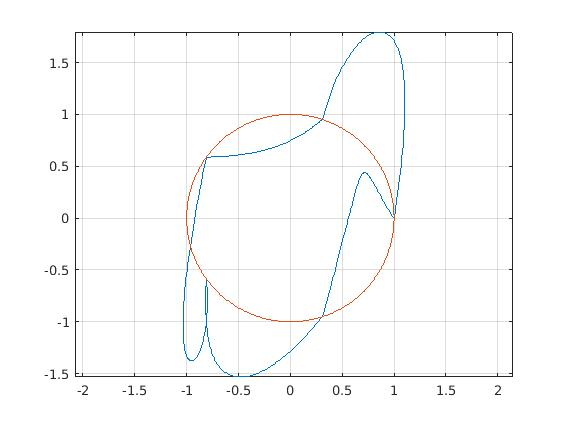
\includegraphics[width = 2.7in]{./stab5.jpg}} \\
\subfloat[N = 10]{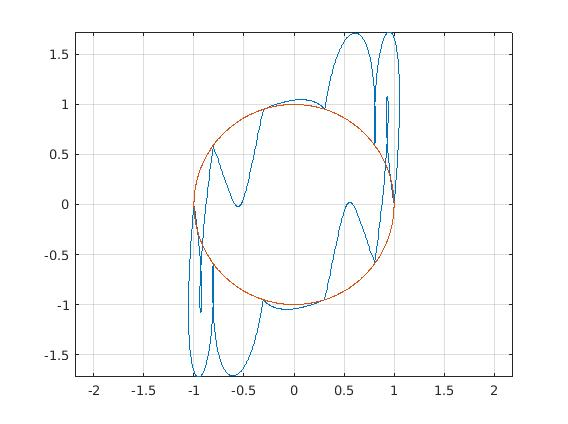
\includegraphics[width = 2.7in]{./stab10.jpg}} &
\subfloat[N = 20]{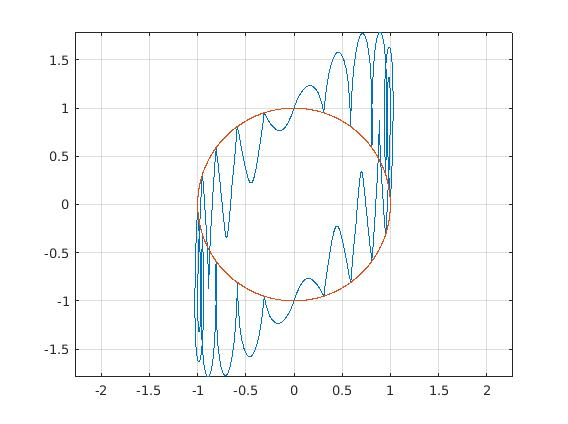
\includegraphics[width = 2.7in]{./stab20.jpg}}\\
\end{tabular}
\caption{}
\end{figure}
\subsection{Results of Simulation for the Unstable System}
Figure 2 contains graphs of the driven system $A_{1}x + Bu$ for various values of $N$. Instead of more closely adhering to the circle, our system states appear to vacillate wildly between points. As shown in section 4, there is no input that causes the system $A_{1}x + Bu$ to trace the unit circle. As we expect, our attempt to drive the system to interpolate the unit circle along an increasing number of samples does not work either. Instead of approximating the circle, our states converge on something else.  We speculate that this occurs because of the internal structure of the system---it's contraction inducing eigenvalues and the eigenvectors along which the contraction occurs.
\pagebreak

\begin{figure}
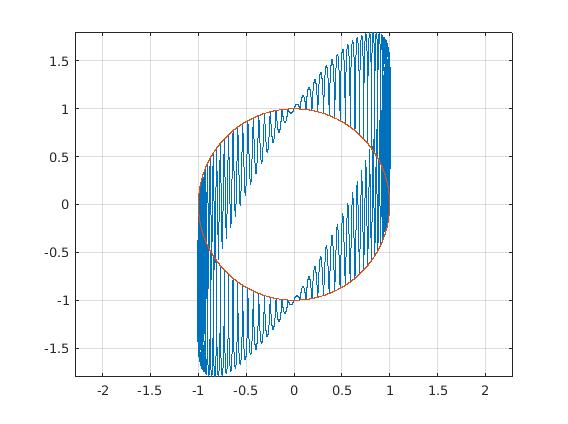
\includegraphics[width=5in]{./stab100.jpg}
\caption{}
\end{figure}
\subsection{Further Work}
Figure 3 shows the stable system when it is driven to interpolate 100 points on the unit circle. Curiously enough, we begin to see the outline of an ellipse. Why does this ellipse appear? What is the reason it is oriented as it is? Can we solve for it's parameterization? We hypothesize that our stable system can trace the shown ellipse in the same way the semi-stable system can trace the unit circle.\\

\noindent Additionally, when we sampled the circle and produced input, we used the minimum energy input to drive our system. This begs the question, What if we used a different input? Is there an input that can drive the stable system to follow the unit circle perfectly? This question can be posed as an optimization problem:\\

Find $u(t)$ such that, 
\[ \| A_{1}x(t)+Bu(t) - \begin{bmatrix} cos(\omega t) \\ -sin(\omega t)\end{bmatrix} \|_{L_{2}}\]
is minimized. \\ 

\noindent In a more general sense we ask, given $\epsilon > 0$ and a curve $\gamma(t)$ in $\mathbb{R}^{n}$, is there an input $u(t)$ such that for any reachable system $Ax+Bu$, (where $A \in \mathbb{R}_{nxn}$ and $B \in \mathbb{R}_{nxq}$) with initial condition $x(0) = \gamma(0)$
\[\|Ax(t)+Bu(t) - \gamma(t)\|_{L_{2}} < \epsilon \] for all $t \in \mathbb{R}$?

\section{Conclusion}

It is clear from our examples, that though a system is reachable, it still exhibits structural limitations that may make it difficult to drive it's states to certain values. Some systems may require more energy to achieve a desired state space outcome It remains to be seen if any reachable system can follow any curve in the state space. More work is needed to answer several interesting questions about the structure of a system and it's ability to trace a given curve.
\end{document}
